\documentclass{article}

\usepackage[top=1.2in,bottom=1.2in,left=1.6in,right=1.6in]{geometry}
\usepackage{amsmath}
\usepackage{amssymb}
\usepackage{tikz}
\usepackage{tikz-cd}
\usepackage{enumerate}
\usepackage{charter}
\usepackage{titlesec}
\usepackage{datetime}
\newdate{date}{12}{06}{2017}

% Section titles

% \titleformat{\section}{\Large\bfseries\filcenter}{\thesection}{0.7em}{}[]
\titleformat{\section}{\large\bfseries\filcenter}{\thesection}{0.5em}{}[]
\titleformat{\subsection}[runin]{\bfseries}{\thesubsection.}{0.5em}{}[]

% Numbering

\numberwithin{equation}{subsection}

% Shortcuts

\renewcommand{\ss}[1]{\subsection{#1}}
\newcommand{\Hom}{\mathrm{Hom}}
\newcommand{\sset}{\mathsf{sSet}}
\newcommand{\C}{\mathcal{C}}
\newcommand{\D}{\mathcal{D}}
\newcommand{\id}{\mathrm{id}}
\newcommand{\h}{\mathrm{h}}
\newcommand{\Map}{\mathrm{Map}}
\renewcommand{\S}{\mathcal{S}}
\renewcommand{\P}{\mathsf{PreSh}}

% Title page

\title{Introduction to $\infty$-categories}
\author{Talk by Marco Robalo at DAGIT 2017\\Typed by Timothy Hosgood}
\date{\displaydate{date}}

\begin{document}

    \maketitle

    \begin{abstract}
        These are a copy of my notes on a talk given by Marco Robalo at Derived Algebraic Geometry in Toulouse (DAGIT) 2017: the content is purely his; the mistakes are all mine.
    \end{abstract}

    \section{Motivation}

        \ss{Idea.}
            An \textbf{$\infty$-category} consists of
            \begin{itemize}
                \item objects;
                \item $1$-morphisms between objects;
                \item $n$-morphisms between $(n-1)$-objects (for $n\geqslant2$);
                \item composition laws for $n$-morphisms ($n\geqslant1$) defined up to higher morphisms;
                \item associativity of compositions up to homotopy.
            \end{itemize}

        \ss{Proto-example.} (Fundamental $\infty$-groupoid)
            For a CW-complex $X$ we have
            \begin{itemize}
                \item objects = points;
                \item $1$-morphisms = homotopies;
                \item $2$-morphisms = homotopies of homotopies;
                \item ... and so on.
            \end{itemize}

        \ss{Problem.}
            No direct definition that is operational and simultaneously close to our intuition/desire (infinitely many axioms!).

        \ss{Solution.}
            Find a model category whose objects serve as models for $\infty$-categories.

        \ss{Modelling.}
            Many classical examples:
            \begin{itemize}
                \item homotopy types can be modelled by topological spaces, simplicial sets, categories, etc.;
                \item homotopy theory of homotopy-commutative $\mathbb{Q}$-algebras can be modelled by dg-algebras;
                \item derived stacks can be modelled by simplicial presheaves.
            \end{itemize}

        \ss{Question.}
            Why so many models?

        \ss{Answer.}
            Dwyer-Kan localisation: every model category has an associated $\infty$-category that captures all the important information.

        \ss{Question.}
            If we have models then why care about $\infty$-categories?

        \ss{Answer.}
            Many reasons:
            \begin{itemize}
                \item not all $\infty$-categories have a model presentation;
                \item no `good enough' definition of functors that relate different models (need an $\infty$-functor between the associated $\infty$-categories);
                \item models for diagrams are not always given by diagrams of models;
                \item proofs and statements become `simpler'.
            \end{itemize}

    \section{Preliminary definitions}

        \ss{Category of simplices.}
            Write $\Delta$ to be the \textbf{category of simplices}:
            \begin{itemize}
                \item $\mathrm{ob}(\Delta) = \{[n]\}_{n\in\mathbb{N}}$ where $[n]=\{0<1<\ldots<n\}$ is the ordered set of natural numbers up to $n$;
                \item $\Hom_\Delta([m],[n])$ is the set of order-preserving maps from $[m]$ to $[n]$.
            \end{itemize}

        \ss{Simplicial notation.}
            We use the following notation:
            \begin{itemize}
                \item $\sset = \mathsf{Set}^{\Delta^\mathrm{op}} = \mathsf{Fun}(\Delta^\mathrm{op},\mathsf{Set})$;
                \item $\Delta[n] = \Hom_\Delta(-,[n])\in\sset$;
                \item $S_n = \Hom_\sset(\Delta[n],S)$ for $S\in\sset$;
                \item $\Lambda^i_n = \Delta[n]\setminus\{\text{interior and the face opposite the }j\text{-th vertex}\}$ is the \textbf{$i$-th horn} (for $n\geqslant2$).
            \end{itemize}
            \[
                \Delta[2] =
                \begin{tikzcd}[row sep=1em,column sep=1em]
                    &1\ar{dr}\ar[Rightarrow]{d}&\\
                    0\ar{ur}\ar{rr}&\,&2
                \end{tikzcd}
                \qquad\Lambda_2^1 =
                \begin{tikzcd}[row sep=1em,column sep=1em]
                    &1\ar{dr}&\\
                    0\ar{ur}&\,&2
                \end{tikzcd}
            \]

        \ss{Nerve.}
            The \textbf{nerve} $N(\C)$ of a category $\C$ is the simplicial set with
            \begin{itemize}
                \item $n$-simplices given by $(x_0\xrightarrow{f_1}x_1\xrightarrow{f_2}\ldots\xrightarrow{f_n}x_n)$ in $\C$;
                \item boundary maps given by composition (or forgetting the first/last object and morphism for the two edge cases);
                \item degeneracy maps given by inserting the identity.
            \end{itemize}

        \ss{Note.}
            There is a set-bijection
            \[
                \{\text{functors }\C\to\D\}\simeq\{\text{simplicial maps }N(\C)\to N(\D)\}.
            \]

        \ss{Lemma.}
            There is an equivalence of categories $X\simeq N(\C)$ if and only if all \emph{inner} horns lift \emph{uniquely}.
            \[
                \begin{tikzcd}
                    \Lambda_n^i \rar \dar[hook] & X\\
                    \Delta[n] \urar[dashed,swap]{\exists!} &
                \end{tikzcd}
                \quad\text{for all }i\in\{1,\ldots,n-1\}
            \]
        \ss{Composition.}
            For example, ``$\Lambda_2^1$ gives composition''.
            \[
                \begin{tikzcd}[row sep=1em,column sep=1em]
                    &x_1\ar{dr}{f_2}&\\
                    x_0\ar{ur}{f_1}\ar[dashed]{rr}{\exists!f_2\circ f_1}&&x_2
                \end{tikzcd}
            \]

        \ss{Associativity.}
            As another example, ``$\Lambda_3^1$ gives associativity'':
            \[
                x_0\xrightarrow{f_1}x_1\xrightarrow{f_2}x_2\xrightarrow{f_3}x_3\text{ in }\C
            \]
            corresponds to
            \[
                \Lambda_2^1\xrightarrow{(f_2,f_1)}N(\C)
                \quad\text{and}\quad
                \Lambda_2^1\xrightarrow{(f_3,f_2)}N(\C)
            \]
            which generate compositions
            \[
                \Delta[2]\xrightarrow{(f_2,f_1)}N(\C)
                \quad\text{and}\quad
                \Delta[2]\xrightarrow{(f_3,f_2)}N(\C).
            \]
            So $(f_3\circ f_2)\circ f_1 = f_3\circ(f_2\circ f_1)$ if and only if we can `fill the back face of the tetrahedron with vertices $x_0$, $x_1$, $x_2$, and $x_3$', i.e. if and only if we can extend $\Lambda_3^1\to N(\C)$ to $\Delta[3]\to N(\C)$.

        \ss{Exercise.}
            What does the lifting of $\Lambda_3^2$ tell us?

        \ss{Summary.}
            The lifting property for inner horns ($0<i<n$) gives composition and associativity laws; for outer horns ($i=0,n$) it gives inverses.
            \[
                \begin{tikzcd}[row sep=1em,column sep=1em]
                    &x_0\ar[dashed]{dr}{\exists!}&\\
                    x_0\ar{ur}{\id_{X_0}}\ar{rr}{f_1}&&x_1
                \end{tikzcd}
            \]

        \ss{Kan complex.}
            If $X\in\sset$ is such that $X\simeq\mathrm{Sing}(T)$, where $\mathrm{Sing}(T)$ consists of singular simplices in a topological space $T$ (i.e. continuous maps $|\Delta^n|\to T$) then we call it a \textbf{Kan complex}.
            Note that $X$ is a Kan complex if and only if \emph{all} horns lift, but \emph{not necessarily} uniquely.

    \section{Quasi-categories}

        \ss{Quasi-category.}
            A \textbf{quasi-category} is a simplicial set $\C$ such that all \emph{inner} horns lift, but \emph{not necessarily} uniquely.
            This notions lies in between that of a Kan complex and that of the nerve of a category: we get compositions that aren't unique, but their non-uniqueness is controlled by higher homotopy data.
            For example, consider
            \[
                x_0\xrightarrow{f_1}x_1\xrightarrow{f_2}x_2\xrightarrow{\id_{x_2}}x_2
            \]
            which gives us two maps $u_1,u_2\colon\Delta[2]\to\C$.
            Similarly, for `associativity' we can use the lifting of $\Lambda_3^1$ as before, after filling one face with the identity.

        \ss{$\infty$-category.}
            We can use quasi-categories as a model for \textbf{$\infty$-categories}: define the objects of a quasi-category $\C$ to be the $0$-simplices, and the $n$-morphisms to be the $n$-simplices.

        \ss{$\infty$-functor.}
            Since functors are `maps that preserve commutative diagrams', it makes sense to define an \textbf{$\infty$-functor} to be a map of simplicial sets between quasi-categories, since these send $n$-simplices to $n$-simplices and preserve boundaries.

        \ss{Homotopy category.}
            Given an $\infty$-category $\C$ we define its \textbf{homotopy category $\h\C$} to be the ($1$-)category with
            \begin{itemize}
                \item $\mathrm{ob}(\h\C)=\mathrm{ob}(\C)$;
                \item $\Hom_{\h\C}(x,y)=\Hom_\C(x,y)\,/\sim$, where $f\sim g$ if there exists a $2$-morphism $u\colon\Delta[2]\to\C$ with boundary $(\id_y-g+f)$.
            \end{itemize}
            \[
                \begin{tikzcd}[row sep=1em,column sep=1em]
                    &y \ar{dr}{\id_y} \ar[Rightarrow]{d}{u}&\\
                    x \ar{ur}{f} \ar[swap]{rr}{g}&\,&y
                \end{tikzcd}
            \]
            Note that compositions are unique (and thus well defined) thanks to the lifting property, i.e. $u_1,u_2$ are identified in the homotopy category.

        \ss{Subcategory.}
            An \textbf{$\infty$-subcategory} $\C'$ of an $\infty$-category $\C$ is a sub-simplicial set obtained as a fibre product in $\sset$:
            \[
                \begin{tikzcd}[row sep=.4em,column sep=0em]
                    \C' \ar{dd}\ar{rr} && \C \ar{dd}\\
                    &\lrcorner&\\
                    N(\mathcal{D}) \ar{rr} && N(\h\C)
                \end{tikzcd}
                \quad\text{where }\mathcal{D}\text{ is a subcategory of }\h\C.
            \]

        \ss{Equivalence.}
            A $1$-morphism $f$ in $\C$ is called an \textbf{equivalence} if $[f]$ in $\h\C$ is an isomorphism.

        \ss{$\infty$-groupoid.}
            An $\infty$-category where \emph{all} $1$-morphisms are equivalences is called an \textbf{$\infty$-groupoid}.

        \ss{Proposition.}
            An $\infty$-category is an $\infty$-groupoid if and only if it is a Kan complex.

        \ss{Example.}
            For $T$ a topological space, $\mathrm{Sing}(T)$ is an $\infty$-groupoid

    \section{Simplicial nerve and rectification}

        \ss{Mapping space.}
            Let $x,y$ be objects in an $\infty$-category $\C$.
            We define the \textbf{mapping space $\Map_\C(x,y)$} as the simplicial set obtained as the fibre product
            \[
                \Delta[0]\times_\C\mathsf{Fun}(\Delta[1],\C)\times_\C\Delta[0]
            \]
            where the maps are given by $x,y\colon\Delta[0]\to\C$ and $\mathrm{ev}_0,\mathrm{ev}_1\colon\mathsf{Fun}(\Delta[1],\C)\to\C$, where $\mathrm{ev}_n$ is the evaluation on $n$.

        \ss{Note.}
            Another notation used is $\Hom_\C^{\mathrm{LR}}(x,y)$, where we write the pullback as
            \[
                \begin{tikzcd}[row sep=.4em,column sep=0em]
                    \Hom_\C^{\mathrm{LR}}(x,y) \ar{dd}\ar{rr} && \C^{\Delta[1]} \ar{dd}\\
                    &\lrcorner&\\
                    \{x\}\times\{y\} \ar{rr} && \C\times\C
                \end{tikzcd}
            \]

        \ss{Proposition.}
            $\Map_\C(x,y)$ is a Kan complex.

        \ss{Note.}
            $\pi_0\Map_\C(x,y)\simeq\Hom_{\h\C}(x,y)$.

        \ss{Warning.}
            These is \emph{no} strict manifestation of composition:
            \[
                \Map_\C(y,z)\times\Map_\C(x,y) \not\to \Map_\C(x,z).
            \]

        \ss{Rectification.} (Lurie)
            There exists $\widetilde{\Map}_\C(x,y)\in\sset$ and \emph{canonical} zig-zags of weak equivalences of simplicial sets
            \[
                \widetilde{\Map}_\C(x,y) \xrightarrow{\sim} \{*\} \xleftarrow{\sim} \Map_\C(x,y)
            \]
            such that we \emph{do} get strict manifestations of composition maps.
            We write $\mathfrak{C}[\C]$ for the \textbf{rectified category}, which is simply $\C$ but with $\widetilde{\Map}$ replacing $\Map$.
            Note that the rectified category is a true simplicial category.

        \ss{Simplicial nerve.}
            There exists a \emph{non-trivial} extension of the nerve construction to simplicial categories that takes into account the simplicial structure, i.e. the \textbf{simplicial nerve} $N_\Delta(\mathcal{E})$ is a simplicial set when $\mathcal{E}$ is a simplicial category.

        \ss{Application.}
            We can model a simplicial category $\mathcal{E}$ by the simplicial set $N_\Delta(\mathcal{E})$.

        \ss{Theorem.} (Joyal-Lurie)
            There exists a model structure on $\sset$ with
            \begin{itemize}
                \item cofibrant-fibrant objects = quasi-categories;
                \item weak equivalences = essentially surjective morphisms that induce a weak equivalence on mapping spaces.
            \end{itemize}

        \ss{Theorem.} (Bergner)
            There exists a model structure on $\mathsf{Cat}^{\Delta^\mathrm{op}}$ with
            \begin{itemize}
                \item cofibrant-fibrant objects = simplicial categories enriched over Kan complexes;
                \item weak equivalences = essentially surjective morphisms that induce a weak equivalence on mapping spaces.
            \end{itemize}

        \ss{Theorem.} (Lurie)
            The adjunction $(\mathfrak{C}\dashv N_\Delta)$ forms a Quillen equivalence.

        \ss{Example.}
            Let $\mathcal{M}$ be a simplicial model category and write $\mathcal{M}^\mathrm{cf}$ to mean the subcategory of cofibrant-fibrant objects.
            Then $\mathcal{M}^\mathrm{cf}$ is enriched over Kan complexes and so $N_\Delta(\mathcal{M}^\mathrm{cf})$ is a quasi-category.

        \ss{Rectification of diagrams.}
            Let $\D$ be a category and $\mathcal{M}$ a combinatorial simplicial model category.
            Then there is an equivalence of quasi-categories
            \[
                \mathsf{Fun}\Big(N(\D),N_\Delta(\mathcal{M}^\textrm{cf})\Big) \simeq N_\Delta\Big((\mathcal{M}^\D)^\mathrm{cf}\Big)
            \]
            where we endow $\mathcal{M}^\D$ with the projective model structure.

        \ss{Explicit examples.}
            The following three examples are prototypical.
            \begin{enumerate}[I.]
                \item The \textbf{$\infty$-category $\S$ of spaces}.
                    This is $\S=N_\Delta(\sset^\mathrm{cf})$ where
                    \begin{itemize}
                        \item $\sset$ has the model structure used to study weak homotopy equivalences etc.;
                        \item the cofibrant-fibrant objects are Kan complexes;
                        \item $\Map_\S(x,y)\simeq\underline{\Hom}_{\Delta}(x,y)$.
                    \end{itemize}
                \item The \textbf{$\infty$-category $\mathsf{Cat}_\infty$ of $\infty$-categories}.
                    This is $\mathsf{Cat}_\infty=N_\Delta(\sset)$ where $\sset$ has the model structure as in Joyal-Lurie, but modified in some way so as to make it a simplicial model category.
                \item The \textbf{$\infty$-category $\P(N(\D))$ of presheaves of spaces}.
                    Here $\D$ is an arbitrary category and $\sset$ has the same model structure as in example I.
                    Then
                    \[
                        \P(N(\D)) = \mathsf{Fun}(N(\D^\mathrm{op}),\S) \simeq \mathsf{Fun}\Big(N(\D^\mathrm{op}), N_\Delta(\sset^\mathrm{cf})\Big) \simeq N_\Delta\Big((\sset^{\D^\mathrm{op}})^\mathrm{cf}\Big).
                    \]
            \end{enumerate}

    \section{Homotopy colimits}

        \ss{Initial object.}
            An \textbf{initial object} is some $\varnothing\in\C$ such that, for all $x\in\C$, the Kan complex $\Map_\C(\varnothing,x)$ is contractible.

        \ss{Slogan.}
            Universal objects are defined up to a contractible space of choices.

        \ss{Cones.}
            Given $K\in\sset$ and an infinity functor $d\colon K\to\C$ we construct a new simplicial set $K^\triangleright$ by formally adding an exterior vertex to $K$.
            Then a \textbf{cone under $d$} is a map of simplicial sets $\tilde{d}\colon K^\triangleright\to\C$ such that $\tilde{d}|_K=d$.
            \[
                K^\triangleright =\,\,
                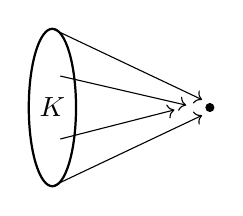
\begin{tikzpicture}[baseline=-0.35em]
                    \draw [thick] (0,0) ellipse (0.3cm and 1cm);
                    \node at (0,0) {$K$};
                    \draw [->] (0,1) -- (1.9,0.1);
                    \draw [->] (0.1,0.4) -- (1.7,0.03);
                    \draw [->] (0.1,-0.4) -- (1.55,.-0.03);
                    \draw [->] (0,-1) -- (1.9,-0.1);
                    \draw [fill] (2,0) circle [radius=0.05];
                \end{tikzpicture}
            \]

        \ss{Proposition.}
            Cones under $d$ give a quasi-category $\C_{d/}$.

        \ss{Colimits.}
            A colimit is an initial object of $\C_{d/}$.

        \ss{Proposition.}
            Let $F\colon\mathcal{J}\to\mathcal{E}$ be a simplicial functor between Kan-enriched categories, and $c\in\mathcal{E}$ an object with a compatible family $\{\eta_{j}\colon F(j)\to c\}$.
            Then $c$ is a \textbf{homotopy colimit of $F$} if and only if the induced map $N_\Delta(\mathcal{J}\to N_\Delta(\mathcal{E})$ is a colimit diagram.

        \ss{Example.}
            \begin{gather*}
                \operatorname{coeq}_{\,\S}\left(
                    *\underset{\id}{\overset{\id}{\rightrightarrows}}*
                \right) \simeq
                \operatorname{colim}_\S\left(
                    \begin{tikzcd}[row sep=1em,column sep=1em,ampersand replacement=\&]
                        *\coprod* \dar\rar \& *\\
                        *
                    \end{tikzcd}
                \right) \simeq
                \operatorname{hocolim}\left(
                    \begin{tikzcd}[row sep=1em,column sep=1em,ampersand replacement=\&]
                        *\coprod* \dar\rar \& *\\
                        *
                    \end{tikzcd}
                \right) \\\simeq
                \operatorname{colim}_\sset\left(
                    \begin{tikzcd}[row sep=1em,column sep=1em,ampersand replacement=\&]
                        *\coprod* \dar\rar \& \Delta[1]\\
                        \Delta[1]
                    \end{tikzcd}
                \right) \simeq
                S^1\in\sset
            \end{gather*}

    \section{Localisation}

    \section{Presheaves and $\infty$-functors}

    \section{Presentability}

    \section{Symmetric monoidal $\infty$-categories}

    \section{Subtleties}

\end{document}
